\documentclass[14pt]{extarticle}
\usepackage[margin=1in]{geometry}
\usepackage{amsmath}
\usepackage{listings}
\usepackage{xcolor}
\usepackage{graphicx}
\usepackage{tcolorbox}
\usepackage{multicol}
\usepackage{titlesec}
\usepackage{enumitem}
\usepackage{titlesec}

% No background color for listings
\lstset{
  basicstyle=\ttfamily\footnotesize,
  frame=single,
  breaklines=true
}


\title{\textbf{Heap Sort}}
\author{Varun Kumar}
\date{July 5, 2025}

\begin{document}
\maketitle 

\subsection*{Constructing Max Heap: Insertion Method vs Build-Heap Method}


\subsection*{1. Key Idea: Insertion Method}
\begin{itemize}
    \item Start with an empty heap.
    \item Insert one element at a time.
    \item After each insertion, perform \textbf{up-heap (bubble up)} to maintain heap property.
\end{itemize}


\subsection*{2. Key Idea: Build-Heap Method}
\begin{itemize}
    \item Start with all elements in array form.
    \item Treat it as a complete binary tree.
    \item Apply \textbf{heapify (down-heap)} from the last non-leaf node up to the root.
\end{itemize}



\vspace{0.5em}
\newpage
\subsection*{Comparisons and Swaps:}
\subsection*{1. Insertion Method}
\begin{itemize}
    \item For each insertion, worst-case comparisons = height of tree = \( \log i \)
    \item Total comparisons: \( O(n \log n) \)
    \item Each insertion may involve several swaps.
\end{itemize}

\subsection*{2. Build-Heap Method}
\begin{itemize}
    \item Heapify from \( \left[ \frac{n}{2} - 1 \right] \) to 0.
    \item Comparisons are fewer near the top.
    \item Total comparisons: \( O(n) \)
    \item Much more efficient than repeated insertion.
\end{itemize}

\vspace{0.5em}

\subsection*{Optimal Behavior}
\begin{itemize}
    \item \textbf{Insertion method:} Intuitive but inefficient for large arrays.
    \item \textbf{Build-heap method:} Optimal and used in Heap Sort.
    \item For \( n \) elements, build-heap runs in \( O(n) \) while insertions take \( O(n \log n) \).
\end{itemize}



\newpage
\subsubsection*{Pseudocode: Insertion Method}
\begin{lstlisting}[language=Python]
insert(heap, value):
    heap.append(value)
    i = len(heap) - 1
    while i > 0:
        parent = (i - 1) // 2
        if heap[i] > heap[parent]:
            swap(heap[i], heap[parent])
            i = parent
        else:
            break
\end{lstlisting}

\vspace{4em}

\subsubsection*{Pseudocode: Build-Heap Method}

\begin{lstlisting}[language=Python]
buildHeap(arr, n):
    for i in range(n//2 - 1, -1, -1):
        heapify(arr, n, i)

heapify(arr, n, i):
    largest = i
    left = 2*i + 1
    right = 2*i + 2

    if left < n and arr[left] > arr[largest]:
        largest = left
    if right < n and arr[right] > arr[largest]:
        largest = right

    if largest != i:
        swap(arr[i], arr[largest])
        heapify(arr, n, largest)
\end{lstlisting}


\vspace{1em}
\newpage
\subsubsection*{Example: Build Max Heap using Insertion Method}

\textbf{Input:} Insert elements one-by-one from: \([3, 5, 1, 10, 2, 7, 6, 4]\)

\begin{enumerate}[leftmargin=*]
    \item Insert 3 → No parent to compare  
        \[
        [3]
        \]

    \item Insert 5  
        \[
        [3, 5] \rightarrow \text{5 > 3} \Rightarrow \text{Swap} \Rightarrow [5, 3]
        \]

    \item Insert 1  
        \[
        [5, 3, 1] \rightarrow \text{1 < 5} \Rightarrow \text{No change}
        \]

    \item Insert 10  
        \[
        [5, 3, 1, 10] \rightarrow \text{10 > 3} \Rightarrow \text{Swap} \Rightarrow [5, 10, 1, 3]
        \]
        \[
        \text{10 > 5} \Rightarrow \text{Swap} \Rightarrow [10, 5, 1, 3]
        \]

    \item Insert 2  
        \[
        [10, 5, 1, 3, 2] \rightarrow \text{2 < 5} \Rightarrow \text{No change}
        \]

    \item Insert 7  
        \[
        [10, 5, 1, 3, 2, 7] \rightarrow \text{7 > 1} \Rightarrow \text{Swap} \Rightarrow [10, 5, 7, 3, 2, 1]
        \]

    \item Insert 6  
        \[
        [10, 5, 7, 3, 2, 1, 6] \rightarrow \text{6 < 7} \Rightarrow \text{No change}
        \]

    \item Insert 4  
        \[
        [10, 5, 7, 3, 2, 1, 6, 4] \rightarrow \text{4 > 3} \Rightarrow \text{Swap} \Rightarrow [10, 5, 7, 4, 2, 1, 6, 3]
        \]
\end{enumerate}

\textbf{Final Max Heap:} \([10, 5, 7, 4, 2, 1, 6, 3]\)


\subsubsection*{Example: Build Max Heap using Heapify}

\textbf{Input:} \([3, 5, 1, 10, 2, 7, 6, 4]\), \(n = 8\)

\begin{enumerate}[leftmargin=*]
    \item Start heapifying from \( i = \lfloor n/2 \rfloor - 1 = 3 \)
    \item \textbf{heapify(3):} 
        \[
        \text{Node: 10, Left: 4, Right: None} \Rightarrow \text{No change}
        \]
    \item \textbf{heapify(2):}
        \[
        \text{Node: 1, Left: 7, Right: 6} \Rightarrow \text{7 > 1} \Rightarrow \text{Swap 1 and 7}
        \]
        New array: \([3, 5, 7, 10, 2, 1, 6, 4]\)

    \item \textbf{heapify(1):}
        \[
        \text{Node: 5, Left: 10, Right: 2} \Rightarrow \text{10 > 5} \Rightarrow \text{Swap 5 and 10}
        \]
        New array: \([3, 10, 7, 5, 2, 1, 6, 4]\)

    \item \textbf{heapify(3):}
        \[
        \text{Node: 5, Left: 4, Right: None} \Rightarrow \text{No change}
        \]

    \item \textbf{heapify(0):}
        \[
        \text{Node: 3, Left: 10, Right: 7} \Rightarrow \text{10 > 3} \Rightarrow \text{Swap 3 and 10}
        \]
        New array: \([10, 3, 7, 5, 2, 1, 6, 4]\)

    \item \textbf{heapify(1):}
        \[
        \text{Node: 3, Left: 5, Right: 2} \Rightarrow \text{5 > 3} \Rightarrow \text{Swap 3 and 5}
        \]
        New array: \([10, 5, 7, 3, 2, 1, 6, 4]\)

    \item \textbf{heapify(3):}
        \[
        \text{Node: 3, Left: 4, Right: None} \Rightarrow \text{4 > 3} \Rightarrow \text{Swap}
        \]
        Final array: \([10, 5, 7, 4, 2, 1, 6, 3]\)
\end{enumerate}

\textbf{Final Max Heap:} \([10, 5, 7, 4, 2, 1, 6, 3]\)


\subsection*{Python code for Max-Heap Construction using Heapify from Middle to Root}
\begin{lstlisting}[language=Python]
def heapify(arr, n, i):
    largest = i           # Assume current index is largest
    left = 2 * i + 1      # Left child index
    right = 2 * i + 2     # Right child index

    # Check if left child exists and is greater than current largest
    if left < n and arr[left] > arr[largest]:
        largest = left

    # Check if right child exists and is greater than current largest
    if right < n and arr[right] > arr[largest]:
        largest = right

    # If largest is not the current index, swap and continue heapifying
    if largest != i:
        arr[i], arr[largest] = arr[largest], arr[i]
        heapify(arr, n, largest)

def build_max_heap(arr):
    n = len(arr)
    # Start from last non-leaf node and move up to root
    for i in range(n//2 - 1, -1, -1):
        heapify(arr, n, i)

# Input array
arr = [3, 5, 1, 10, 2, 7, 6, 4]
print("Before-Build-Heap:", arr)
build_max_heap(arr)
print("After Build-Heap:", arr)

\end{lstlisting}

\subsection*{Is Build-Heap Method Stable? If No, then why?}

\textbf{Answer:} \textbf{No}, the Build-Heap Method is \textbf{not stable}.

\begin{itemize}
    \item It uses \texttt{heapify()} which swaps elements without checking their original position.
    \item On equal values, it may move the element that appeared earlier in the input to a lower position in the heap.
    \item This violates the principle of stability: \textit{"equal elements retain their original order"}.
\end{itemize}


\vspace{1em}

\subsubsection*{Example of Instability in Build-Heap}

Input with tagged equal elements:

\[
\texttt{[(4a), (3), (4b)]}
\]

\begin{itemize}
    \item Initial positions: \texttt{4a} before \texttt{4b}
    \item When heapify is called at index 0:
        \begin{itemize}
            \item Children: \texttt{4b} and \texttt{3}
            \item Heapify may choose \texttt{4b} (right child) over \texttt{4a} (root)
            \item After swap: \texttt{[(4b), (3), (4a)]}
        \end{itemize}
    \item Now \texttt{4b} appears before \texttt{4a} — original order broken.
\end{itemize}

\textbf{Hence, Build-Heap is not stable.}

\subsection*{Why Heap Sort is Unstable}

Heap Sort is \textbf{not stable} because it may change the relative order of equal elements.

\subsubsection*{Unstable Operation: \texttt{swap()} in \texttt{heapify()}}

\subsection*{Root Cause of Instability}
\begin{itemize}
    \item During the \texttt{heapify()} process in \texttt{buildHeap()}, nodes are compared and swapped.
    \item If two elements have the \textbf{same value}, their \textbf{original order can be reversed} by swapping.
    \item This violates the definition of a stable sort.
\end{itemize}
\newpage
\subsubsection*{Example: Loss of Stability}

Consider the input array with values and tags:

\[
[(4, \text{A}),\ (3, \text{B}),\ (4, \text{C})]
\]

\begin{itemize}
    \item Both elements A and C have value 4.
    \item After applying heapify, the element \texttt{(4, C)} may be moved above \texttt{(4, A)}.
    \item This reverses their original order and makes the sort unstable.
\end{itemize}

\subsubsection*{How to Make Build-Heap Stable? Stable Heap Suggestion}
To preserve stability:
\begin{itemize}
    \item During comparisons, compare tuples: \texttt{(value, original\_index)}
    \item If two elements have the same value, prefer the one with the \textbf{smaller original index}.
    \item This avoids swapping equal elements out of order.
\end{itemize}


\noindent
Thus, standard \texttt{buildHeap()} is unstable due to arbitrary swaps of equal values. To fix this, we must track and respect original positions.


\vspace{1em}

\subsubsection*{Modified Comparison Example}

\[
\texttt{[(4, 0), (3, 1), (4, 2)]}
\]

\begin{itemize}
    \item Compare \texttt{(4, 0)} and \texttt{(4, 2)}:
        \begin{itemize}
            \item Values equal: \(4 = 4\)
            \item Use index: \(0 < 2\) → keep \texttt{(4, 0)} above
        \end{itemize}
    \item Thus, original order is preserved.
\end{itemize}

\vspace{1em}

\textbf{Note:} This requires more memory (to store index) and slightly slower comparisons, but gives \textbf{stability}.



\newpage
\subsection*{Python code for Max-Heap Construction using Insertion Method}
\begin{lstlisting}[language=Python]
def insert_max_heap(heap, value):
    heap.append(value)  # Add new value at the end
    i = len(heap) - 1   # Index of inserted value

    # Bubble up (up-heap) to maintain max-heap property
    while i > 0:
        parent = (i - 1) // 2
        if heap[i] > heap[parent]:
            # Swap if child is greater than parent
            heap[i], heap[parent] = heap[parent], heap[i]
            i = parent
        else:
            break

# Input array
arr = [3, 5, 1, 10, 2, 7, 6, 4]
heap = []

print("Step-by-step insertion into Max-Heap:")
for val in arr:
    insert_max_heap(heap, val)
    print(heap)

\end{lstlisting}

\subsection*{Is Insertion based Heap Sort Stable? If no, then why?}

\textbf{Answer:} \textbf{No}, Heap Sort is \textbf{not stable}.

\begin{itemize}
    \item \textbf{Heapify} and \textbf{swap} operations reorder elements based on value only.
    \item They do \textbf{not preserve the original order} of equal elements.
    \item This violates the condition of stability.
\end{itemize}

\newpage
\subsubsection*{Example Demonstrating Instability}

Assume elements have labels to distinguish duplicates:

\begin{itemize}
    \item Input array: \texttt{[(5a), 4, (5b), 3]}
    \item Note: \texttt{5a} and \texttt{5b} have equal values but different initial positions.
\end{itemize}

\textbf{Step: Build Max Heap}
\begin{itemize}
    \item Heapify at index 1: no change
    \item Heapify at index 0:
        \begin{itemize}
            \item Compares \texttt{5a} (index 0) and \texttt{5b} (index 2)
            \item May pick \texttt{5b} as root (due to implementation order)
        \end{itemize}
\end{itemize}

\textbf{Resulting Heap:} \texttt{[(5b), 4, (5a), 3]}

\textbf{Conclusion:} Relative order of equal elements \texttt{5a}, \texttt{5b} is changed.

\vspace{1em}

\subsection*{Which Operation Causes Instability?}
\textbf{heapify()}:
\begin{itemize}
    \item Selects the largest among parent, left, right — no regard for original position.
    \item On tie (equal values), any child may be chosen.
    \item This leads to non-stable reordering.
\end{itemize}


\vspace{1em}

\subsubsection*{Can Heap Sort be Made Stable?}

\begin{itemize}
    \item Yes, by storing a tuple \texttt{(value, original\_index)}.
    \item Modify comparisons to break ties using index.
    \item But this is not standard Heap Sort anymore.
\end{itemize}

\subsection*{Time Complexity of Heap Sort}

\begin{itemize}
    \item \textbf{Best Case:} \( O(n \log n) \)
    \begin{itemize}
        \item Even in the best scenario, Heap Sort does not benefit from partial ordering.
        \item Every element still needs to be heapified and extracted.
    \end{itemize}

    \item \textbf{Average Case:} \( O(n \log n) \)
    \begin{itemize}
        \item On average, heap construction takes \( O(n) \) and each of the \( n \) extractions takes \( O(\log n) \).
    \end{itemize}

    \item \textbf{Worst Case:} \( O(n \log n) \)
    \begin{itemize}
        \item In the worst case, all heapify operations go to the bottom of the tree.
        \item Each delete-max operation takes \( O(\log n) \).
    \end{itemize}
\end{itemize}

\vspace{0.5em}

\subsection*{Space Complexity}
\begin{itemize}
    \item \textbf{Auxiliary Space:} \( O(1) \) (in-place sorting)
\end{itemize}
\subsection*{Heap Sort Summary Table}

\begin{center}
\renewcommand{\arraystretch}{1.4}
\begin{tabular}{|c|c|c|c|c|c|}
\hline
\textbf{Case} & \textbf{Comparisons} & \textbf{Swaps} & \textbf{Time} & \textbf{Adaptive} & \textbf{Stable} \\
\hline
Best Case & \( O(n \log n) \) & \( O(n \log n) \) & \( O(n \log n) \) & No & No \\
\hline
Average Case & \( O(n \log n) \) & \( O(n \log n) \) & \( O(n \log n) \) & No & No \\
\hline
Worst Case & \( O(n \log n) \) & \( O(n \log n) \) & \( O(n \log n) \) & No & No \\
\hline
\end{tabular}
\end{center}

\newpage
\section{GATE CSE 2004}
The elements $32, 15, 20, 30, 12, 25, 16$ are inserted one by one in the given order into a maxHeap.
The resultant maxheap is

\begin{enumerate}[label=(\alph*)]

    \item 
    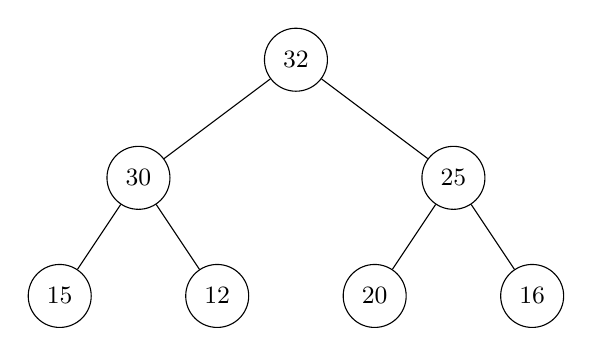
\begin{tikzpicture}[
      level 1/.style={sibling distance=40mm},
      level 2/.style={sibling distance=20mm},
      every node/.style={circle, draw, minimum size=8mm, font=\small}
    ]
    \node{32}
      child {node{30}
        child {node{15}}
        child {node{12}}
      }
      child {node{25}
        child {node{20}}
        child {node{16}}
      };
    \end{tikzpicture}

    \item 
    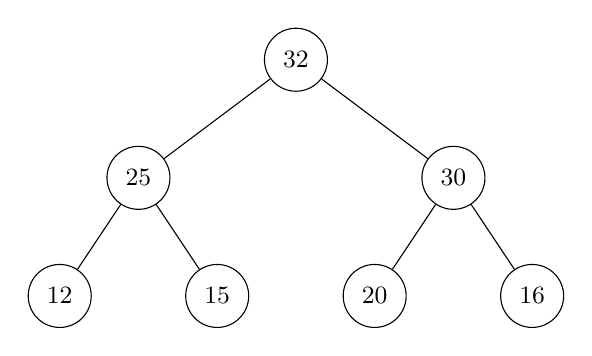
\begin{tikzpicture}[
      level 1/.style={sibling distance=40mm},
      level 2/.style={sibling distance=20mm},
      every node/.style={circle, draw, minimum size=8mm, font=\small}
    ]
    \node{32}
      child {node{25}
        child {node{12}}
        child {node{15}}
      }
      child {node{30}
        child {node{20}}
        child {node{16}}
      };
    \end{tikzpicture}

    \item 
    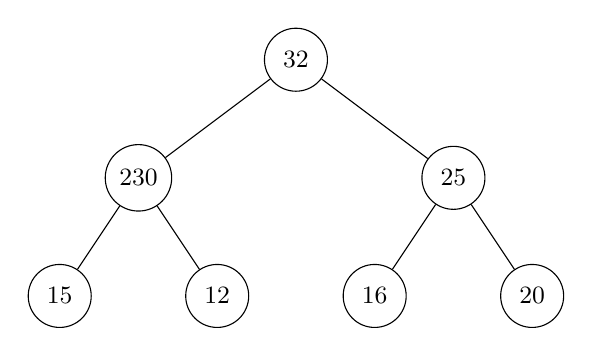
\begin{tikzpicture}[
      level 1/.style={sibling distance=40mm},
      level 2/.style={sibling distance=20mm},
      every node/.style={circle, draw, minimum size=8mm, font=\small}
    ]
    \node{32}
      child {node{230}
        child {node{15}}
        child {node{12}}
      }
      child {node{25}
        child {node{16}}
        child {node{20}}
      };
    \end{tikzpicture}

    \item 
    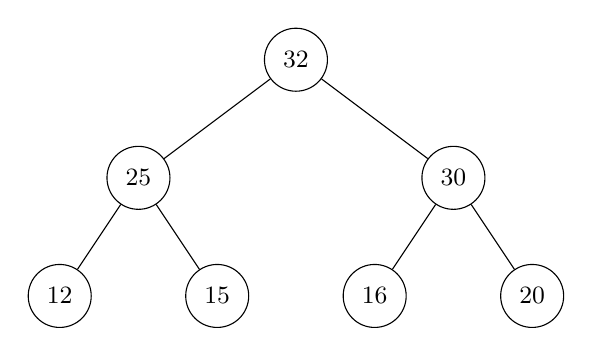
\begin{tikzpicture}[
      level 1/.style={sibling distance=40mm},
      level 2/.style={sibling distance=20mm},
      every node/.style={circle, draw, minimum size=8mm, font=\small}
    ]
    \node{32}
      child {node{25}
        child {node{12}}
        child {node{15}}
      }
      child {node{30}
        child {node{16}}
        child {node{20}}
      };
    \end{tikzpicture}

\end{enumerate}

\end{document}
